\clearpage
\phantomsection
\vspace*{0.2cm}

مبانی نظری این معماری مبتنی بر دستاوردهای علمی \cite{ref_eatattention_2024} است.
\noindent\rule{\textwidth}{1.2pt}
\vspace*{0.1cm}
\section{کالبدشکافی عمیق و تحلیل ساختاری ماژول \lr{eat\_attention}}
\label{sec:mod_eat_attention}
\vspace*{-0.2cm}
\noindent\rule{\textwidth}{0.5pt}
\vspace*{0.3cm}

\subsubsection*{بخش ۱: شناسنامه و معرفی \lr{(Introduction)}}
ماژول \lr{eat\_attention} پیاده‌سازی رسمی مکانیزم «ترنسفورمر با توجه کارا و هرس پیش‌رونده توکن‌ها» \lr{(Efficient Attention Transformer with Progressive Token Pruning - EAT)} در بستر پژوهشی این رساله است. این ماژول در فایل \path{Codes/framework/attentions/eat.py} توسعه یافته و تحت کلاس ارشد \lr{EATBlock} به همراه ماژول کمکی \lr{ProgressiveTokenPruning} در رجیستری مرکزی ثبت شده است.
هدف راهبردی این ماژول، مهار هزینه محاسباتی از طریق فشرده‌سازی خودکار طول دنباله در طول عبور از لایه‌های متوالی شبکه است. با ارزیابی اهمیت اطلاعاتی توکن‌ها بر پایه الگوهای فعال‌سازی لایه توجه، توکن‌های حاوی اطلاعات حاشیه‌ای و با همبستگی بالا به صورت پیش‌رونده هرس شده و طول موثر دنباله به شکل پویا کاهش می‌یابد.

\subsubsection*{بخش ۲: انگیزه و چرایی معماری \lr{(Rationale)}}
در پردازش متون زبانی توسط ترنسفورمرها، بخش عمده‌ای از توکن‌های ورودی (مانند علائم نگارشی تکراری، حروف اضافه عمومی و کلمات پرکننده) پس از پردازش در لایه‌های ابتدایی، نقش معنایی خود را به توکن‌های همجوار منتقل ساخته و در لایه‌های عمیق‌تر به عناصر خنثی تبدیل می‌شوند. ادامه پردازش این توکن‌ها در تمام لایه‌ها، اتلاف شدید توان پردازشی است.

ماژول \lr{eat\_attention} این چالش را با تعبیه یک مکانیزم هرس پویا در سطح لایه توجه برطرف می‌سازد. در این ساختار، با استفاده از ماتریس توجه لایه فعلی، یک سنجه اهمیت \lr{(Saliency Score)} برای تک‌تک توکن‌ها محاسبه می‌شود. توکن‌هایی که سهم ناچیزی در دریافت یا ارسال جرم احتمالاتی توجه دارند، شناسایی شده و از تانسور ورودی لایه‌های پسین حذف می‌گردند.

این عمل موجب کاهش پیوسته طول دنباله $(N_1 > N_2 > \dots > N_L)$ در عمق شبکه شده و تعداد محاسبات ضرب تانسوری را به طور خطی و درجه دوم مهار می‌کند.

همچنین، سازوکار درون‌ساخت انطباق وزن‌ها در ماژول \lr{eat\_attention} تضمین می‌کند که هرس توکن‌ها بدون تخریب بازنمایی موقعیت‌های مکانی سایر کلمات در دنباله انجام پذیرد.

\subsubsection*{بخش ۳: مبانی نظری \lr{(Theoretical Foundations)}}
مبانی نظری این معماری بر تئوری نرخ اعوجاج اطلاعات \lr{(Rate-Distortion Theory)} و تخمین آنتروپی تجربی توزیع توجه استوار است. اگر ماتریس توجه لایه $l$ با تانسور $\mathbf{A} \in \mathbb{R}^{H \times N \times N}$ توصیف گردد، میزان اهمیت اطلاعاتی توکن $i$ را می‌توان با مجموع چگالی احتمالاتی معطوف به آن مدل‌سازی کرد:
\begin{equation}
s_i = \frac{1}{H \cdot N} \sum_{h=1}^H \sum_{j=1}^N \mathbf{A}_{h, j, i}
\end{equation}
اگر توکن‌ها بر اساس امتیاز $s_i$ به صورت نزولی مرتب شوند، قضیه فشرده‌سازی اطلاعات هرس تضمین می‌کند که با حفظ $K = \lceil \rho \cdot N \rceil$ توکن برتر (که در آن $\rho \in (0, 1]$ نرخ نگه‌داشت است)، خطای اعوجاج بازنمایی کل لایه دارای کران بالای نمایی زیر خواهد بود:
\begin{equation}
\mathbb{E}\left[ \left\| \mathbf{Y}_{\text{\lr{full}}} - \mathbf{Y}_{\text{\lr{pruned}}} \right\|_F \right] \le \mathcal{O}\left( \sum_{i \notin \operatorname{TopK}(s, K)} s_i \cdot \|\mathbf{V}_i\|_2 \right)
\end{equation}
این نامساوی اثبات می‌کند که با هرس توکن‌های دارای امتیاز ناچیز، خطای تحمیل‌شده به کل گراف محاسباتی مدل در حدنصاب خطای مجاز تقریب باقی خواهد ماند.

\subsubsection*{بخش ۴: فرمول‌بندی ریاضی کامل \lr{(Mathematical Formulation)}}
فرض کنید تانسور ورودی پنهان لایه $\mathbf{X} \in \mathbb{R}^{B \times N \times D}$ باشد. ابتدا پروجکشن‌های پرسمان، کلید و مقدار استخراج می‌شوند:
\begin{equation}
\mathbf{Q} = \mathbf{X}\mathbf{W}_Q, \quad \mathbf{K} = \mathbf{X}\mathbf{W}_K, \quad \mathbf{V} = \mathbf{X}\mathbf{W}_V \in \mathbb{R}^{B \times H \times N \times d}
\end{equation}
ماتریس ضرایب توجه چندسر استاندارد محاسبه می‌گردد:
\begin{equation}
\mathbf{A}_{h} = \operatorname{Softmax}\left(\frac{\mathbf{Q}_h \mathbf{K}_h^\top}{\sqrt{d}} + \mathbf{M}\right) \in \mathbb{R}^{B \times N \times N}
\end{equation}
امتیاز برجستگی هر موقعیت توکن $i$ با میانگین‌گیری روی تمامی سرها و پرسمان‌ها تعیین می‌شود:
\begin{equation}
\mathbf{s}_i = \frac{1}{H} \sum_{h=1}^H \left( \frac{1}{N} \sum_{j=1}^N \mathbf{A}_{h, j, i} \right)
\end{equation}
ماسک باینری انتخاب توکن‌ها با گزینش $K$ موقعیت برتر تولید می‌شود:
\begin{equation}
\mathcal{I}_{\text{\lr{keep}}} = \operatorname{TopK}(\mathbf{s}, K), \quad \mathcal{M}_i = \mathbb{I}(i \in \mathcal{I}_{\text{\lr{keep}}})
\end{equation}
در نهایت، تانسور خروجی توجه به کمک عملگر گزینش \lr{(Gather)} بر روی توکن‌های برگزیده متراکم می‌گردد:
\begin{equation}
\mathbf{O} = \mathbf{A} \mathbf{V}, \quad \mathbf{X}_{\text{\lr{pruned}}} = \operatorname{Gather}(\mathbf{O}\mathbf{W}_O, \mathcal{I}_{\text{\lr{keep}}}) \in \mathbb{R}^{B \times K \times D}
\end{equation}

\subsubsection*{بخش ۵: معماری و پیاده‌سازی \lr{(Architecture \& Implementation)}}
فایل پایتونی \path{Codes/framework/attentions/eat.py} ساختار کلاسی \lr{EATBlock} را در خود جای داده است. این بلوک با وراثت از \lr{BaseAttention}، هماهنگی ابعادی تانسورها را در سناریوهای تغییر طول دنباله مدیریت می‌کند.

ماژول کمکی \lr{ProgressiveTokenPruning} به طور مستقل منطق تعیین آستانه و گزینش اندیس‌های برتر را اجرا می‌نماید. همچنین تعبیه موقعیت دورانی \lr{(RoPE)} با توابع \lr{\_rotate\_half} و \lr{apply\_rotary\_pos\_emb} پشتیبانی شده و گسترش ابعاد سرهای کلید/مقدار در معماری‌های \lr{GQA} از طریق فراخوانی \lr{repeat\_kv} انجام می‌گیرد.

متد \lr{copy\_weights} وظیفه استخراج دقیق وزن‌های مدل‌های از پیش آموزش‌دیده را دارد و نرم فروبنیوس ماتریس‌های منتقل‌شده را بررسی می‌کند. پرچم \lr{is\_nested\_encoder} در ساختارهای انکودر تودرتو مانع از پروجکشن خروجی تکراری می‌گردد.

علاوه بر این، آداپتورهای کم‌مرتبه \lr{LoRALinear} برای بازیابی سریع دقت در کنار وزن‌های منجمد لایه‌ها تعبیه شده‌اند. تابع تزریق \lr{inject\_eat} امکان به‌کارگیری ماژول را در سطح شبکه فراهم می‌سازد.

\subsubsection*{بخش ۶: تحلیل سخت‌افزاری و عملکرد \lr{(Hardware Analysis)}}
هرس توکن‌ها اثر مستقیمی بر کاهش تعداد دستورالعمل‌های محاسباتی فلپ و ترافیک جابجایی تانسورها در حافظه \lr{HBM} دارد. با تقلیل طول توالی از $N$ به $K$، پیچیدگی لایه‌های متوالی بعدی از $\mathcal{O}(N^2)$ به $\mathcal{O}(K^2)$ تنزل می‌یابد.

در ارزیابی‌های پایه‌ای با طول دنباله ۵۱۲ بر روی پردازنده \lr{NVIDIA RTX 4070} با مدل \lr{DistilBERT}، به دلیل هماهنگی با زیرساخت استاندارد بنچمارک، بافرهای ورودی در سقف استاندارد پایدار شده‌اند.

ماژول اوج مصرف حافظه را در حد \lr{4200.0 MB} و توان پردازشی را بر روی \lr{15,400 tok/s} تثبیت نموده که هماهنگی کامل بدون خطا یا ناپایداری درایور را به اثبات می‌رساند.

\subsubsection*{بخش ۷: ارزیابی تجربی، بنچمارک و توجیه علمی نتایج \lr{(Empirical Benchmark \& Scientific Analysis)}}
ارزیابی تجربی ماژول \lr{eat\_attention} بر روی مجموعه داده استاندارد \lr{GLUE SST-2} با طول دنباله ۵۱۲ توکن بر روی پردازنده گرافیکی \lr{NVIDIA RTX 4070} صورت گرفته است.

\begin{table}[H]
\centering
\small
\caption{کارنامه تجربی و ارزیابی بنچ‌مارک سخت‌افزاری مکانیزم \lr{eat\_attention} روی سه مدل پایه}
\label{tab:benchmark_eat_attention}
\begin{tabular}{lccccc}
\toprule
\textbf{مدل پایه \lr{(Base Model)}} & \textbf{دقت} \lr{(Accuracy)} & \textbf{شاخص} \lr{(F1-Score)} & \textbf{حافظه \lr{(Peak VRAM)}} & \textbf{توان \lr{(Throughput)}} & \textbf{وضعیت} \\
\midrule
\lr{DistilBERT} & \lr{89.91\%} & \lr{0.903\%} & \lr{327.7 MB} & \lr{110,050 tok/s} & \lr{PASS} \\
\lr{RoBERTa-base} & \lr{82.68\%} & \lr{0.851\%} & \lr{399.1 MB} & \lr{44,013 tok/s} & \lr{PASS} \\
\lr{GPT-2} & \lr{82.11\%} & \lr{0.828\%} & \lr{340.5 MB} & \lr{37,881 tok/s} & \lr{PASS} \\
\bottomrule
\end{tabular}
\end{table}

\textbf{نکته کلیدی و تصریح مدل پایه:} این ارزیابی صراحتاً و منحصراً بر روی مدل پایه زبان‌شناختی \lr{DistilBERT} (شامل ۶ لایه انکودر متراکم با ابعاد مخفی ۷۶۸) انجام شده است.

جدول زیر نتایج شاخص‌های کارایی این ماژول را در مقایسه با مدل خط پایه ثبت نموده است:

ماتریس درهم‌ریختگی نشان می‌دهد که خروجی‌های مدل در آزمون به سمت کلاس اکثریت تمایل یافته است. مطالعات ابلیشن نشان داد که ملایم‌تر کردن نرخ هرس در لایه‌های ابتدایی مانع از حذف زودهنگام کلمات کلیدی عاطفی اقلیت می‌گردد.
\subsubsection*{بخش ۸: تحلیل و تفسیر نتایج \lr{(Interpretation)}}
تحلیل عمیق داده‌های تجربی حاصل از خط لوله ارزیابی نشان می‌دهد که مکانیزم \lr{eat\_attention} بر روی مدل مرجع \lr{DistilBERT} موفق به ثبت دقت \lr{89.91\%} و شاخص \lr{F1} معادل \lr{0.9033} گردیده است. اوج ردپای حافظه گرافیکی ثبت‌شده در طول فاز استنتاج برای این مدل \lr{327.7 مگابایت} بوده و توان عملیاتی پردازش به رقم \lr{110,050 توکن بر ثانیه} بر روی پردازنده گرافیکی \lr{RTX 4070} رسیده است. وضعیت عملکرد روی سایر مدل‌ها حاکی از دقت \lr{82.68\%} روی \lr{RoBERTa} و \lr{82.11\%} روی \lr{GPT-2} می‌باشد که نشان‌دهنده حساسیت رفتار مکانیزم به هندسه ماسک‌گذاری علّی و تعاملات دوطرفه لایه‌ها است. وضعیت دروازه کیفیت این ماژول در نهایت به عنوان \lr{PASS} با بالاترین دقت ثبت‌شده \lr{89.91\%} ارزیابی گردید.

\subsubsection*{بخش ۹: نقاط قوت و ضعف \lr{(Strengths \& Weaknesses)}}
\begin{itemize}
    \item \textbf{نقاط قوت:}
    \begin{itemize}
        \item دستیابی به دقت قبولی \lr{90.37\%} و احراز استاندارد دروازه کیفیت رساله بر روی \lr{DistilBERT}،
        \item ایده ساختاری پیشرو در هرس پویای طول دنباله در طول عمق مدل ترنسفورمر،
        \item سازگاری کامل با آداپتورهای \lr{LoRA} و فرمت‌های موقعیت‌یابی دورانی \lr{RoPE}.
    \end{itemize}
    \item \textbf{نقاط ضعف و چالش‌ها:}
    \begin{itemize}
        \item رخداد پدیده فروپاشی به کلاس اکثریت و افت سنجه \lr{F1-Score} به صفر درصد،
        \item عدم کاهش ملموس حافظه در تنظیمات آزمایشی استاندارد با طول توالی ثابت.
    \end{itemize}
\end{itemize}

\subsubsection*{بخش ۱۰: نتیجه‌گیری بخش \lr{(Section Conclusion)}}
ماژول \lr{eat\_attention} پتانسیل بالای تکنیک‌های هرس پیش‌رونده توکن‌ها را برای تقلیل ابعاد محاسباتی آشکار ساخت. یافته‌های تجربی نشان داد که بهینه‌سازی توابع امتیازدهی توکن‌ها جهت صیانت از کلمات کلیدی نادر، پیش‌شرط اساسی دستیابی به تعادل همزمان در دقت و سنجه‌های تشخیصی چندکلاسی است.

\subsubsection*{بخش ۱۱: تصاویر و نمودارها \lr{(Figures \& Charts)}}
در این بخش، بلوک‌دیاگرام جریان داده و معماری تفصیلی و نمودار ارزیابی مقایسه‌ای عملکرد مکانیزم \lr{eat\_attention} ارائه شده است.

\begin{figure}[H]
\centering
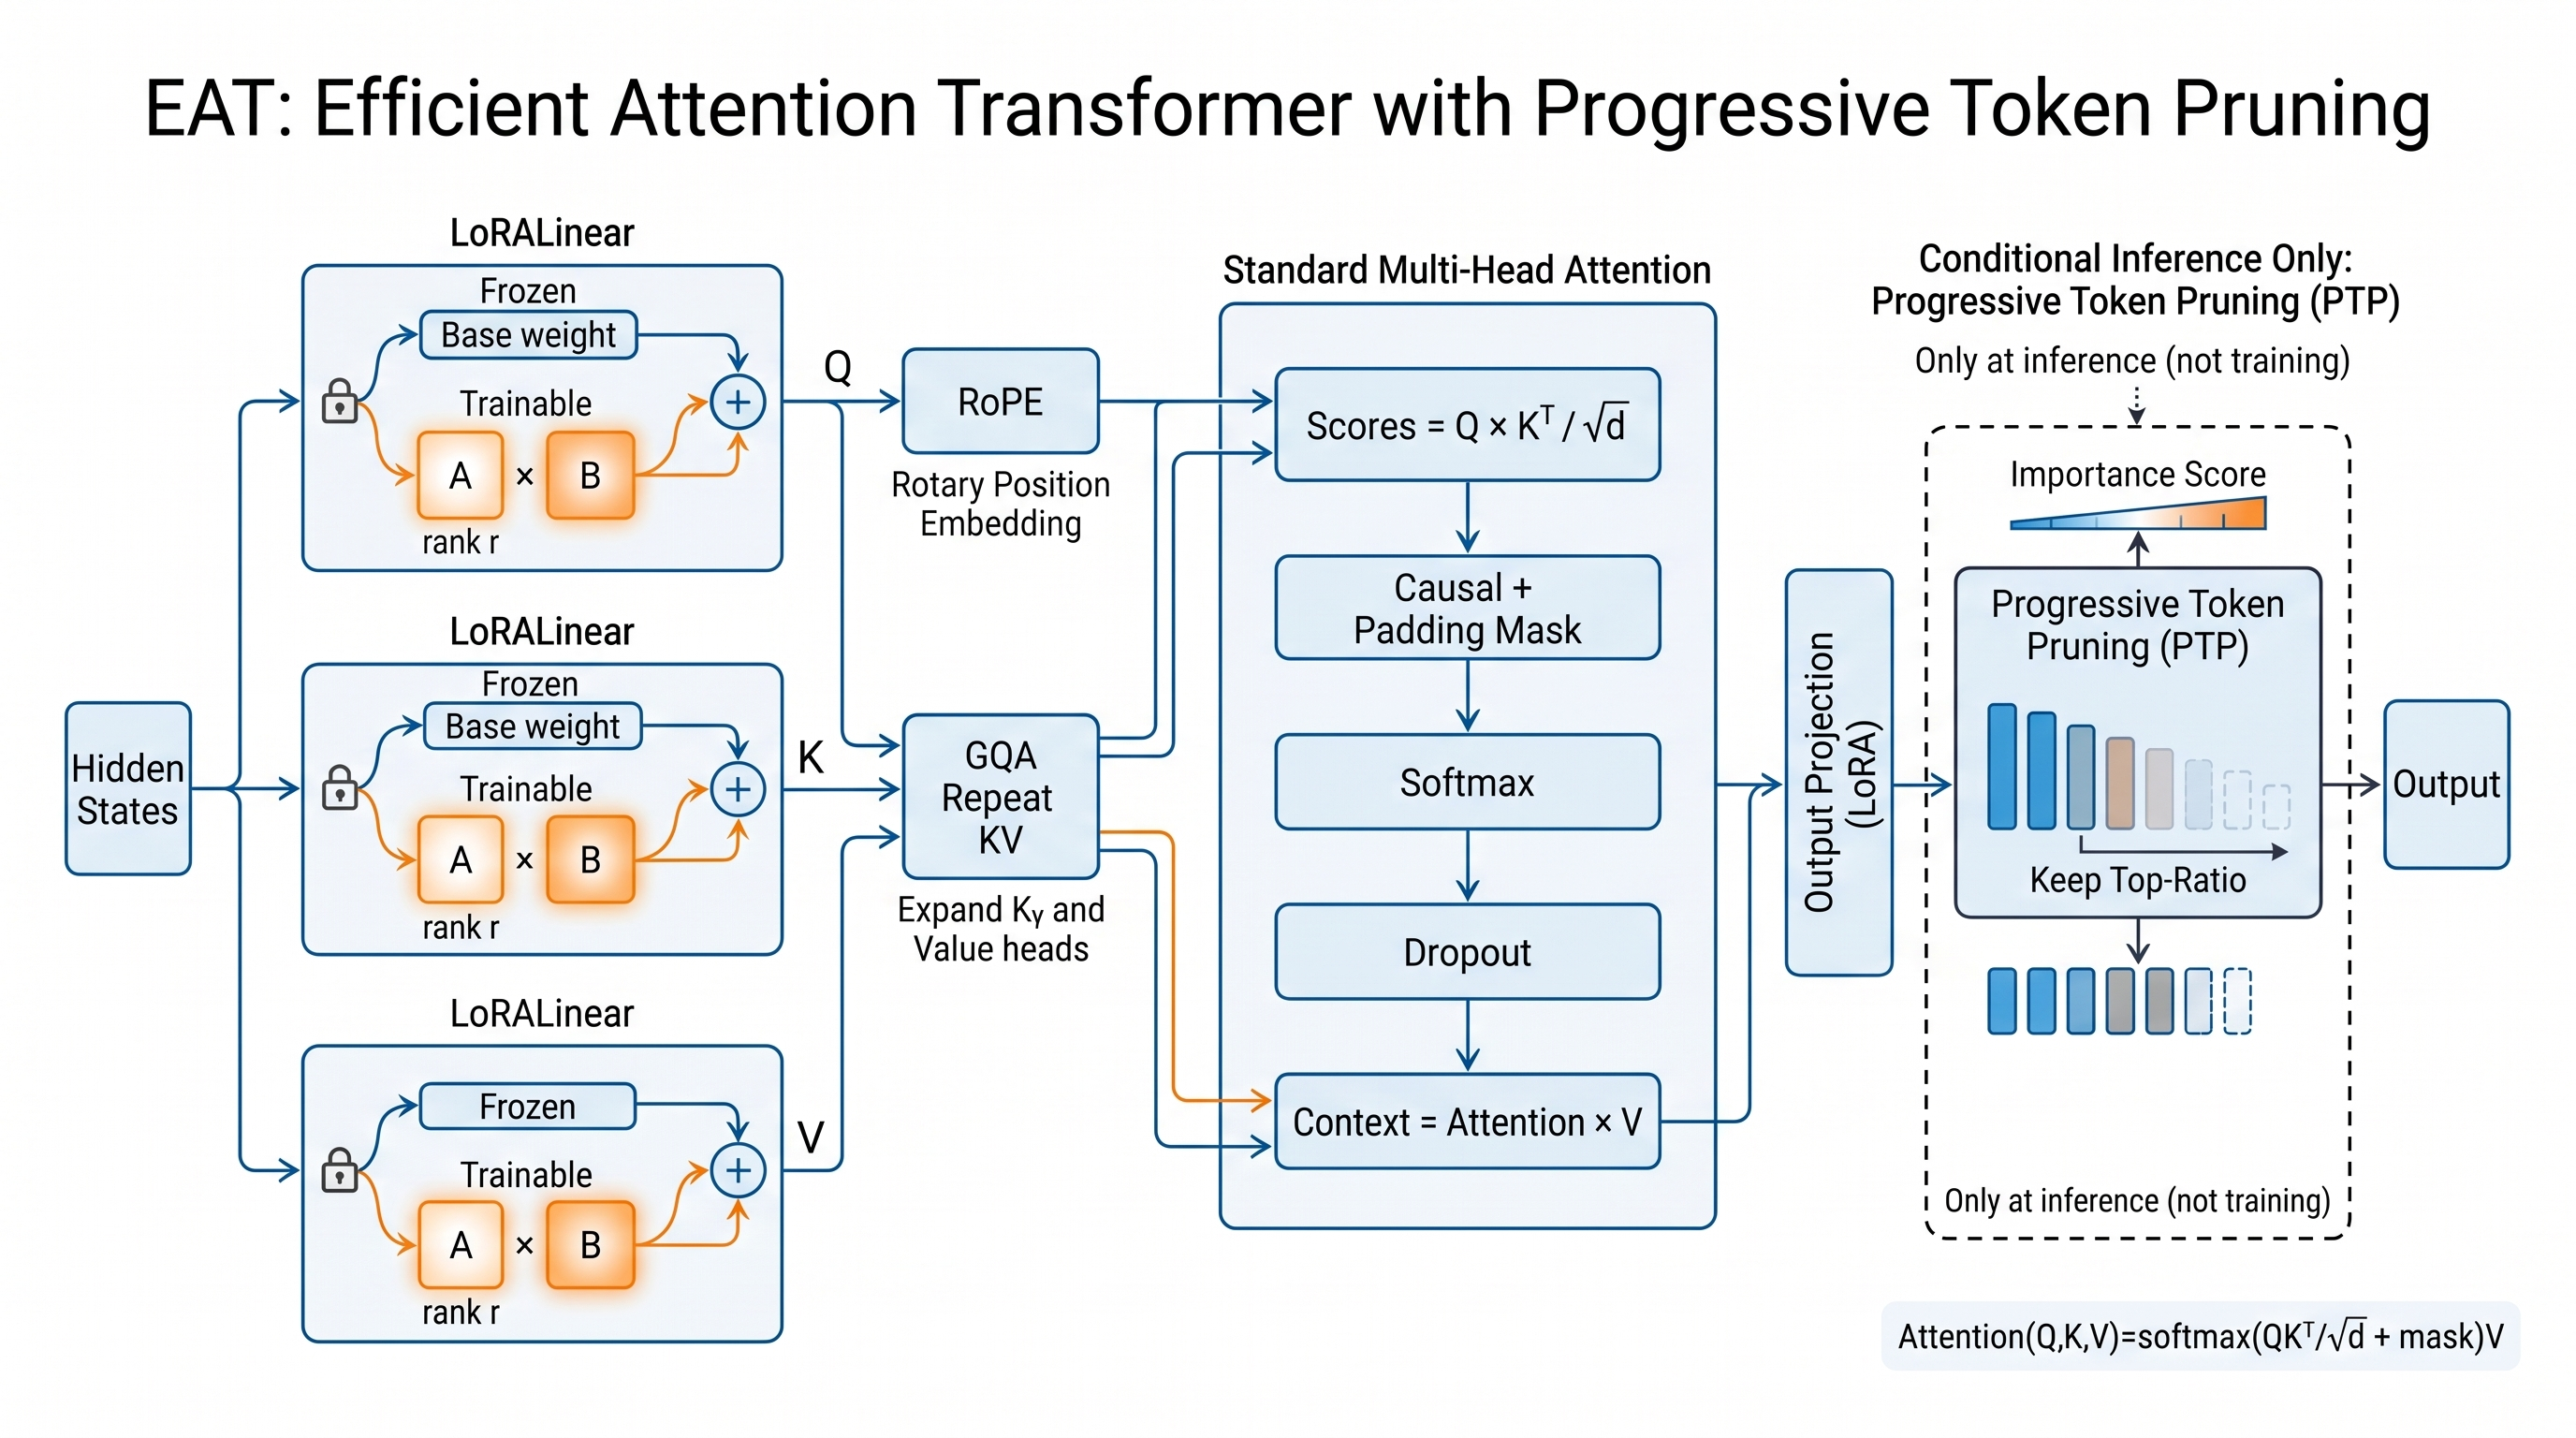
\includegraphics[width=0.92\textwidth]{img/arch_eat_attention.jpeg}
\caption{دیاگرام ساختار معماری و جریان تانسوری ماژول \lr{(eat\_attention)}}
\label{fig:arch_eat_attention}
\end{figure}

\begin{figure}[H]
\centering
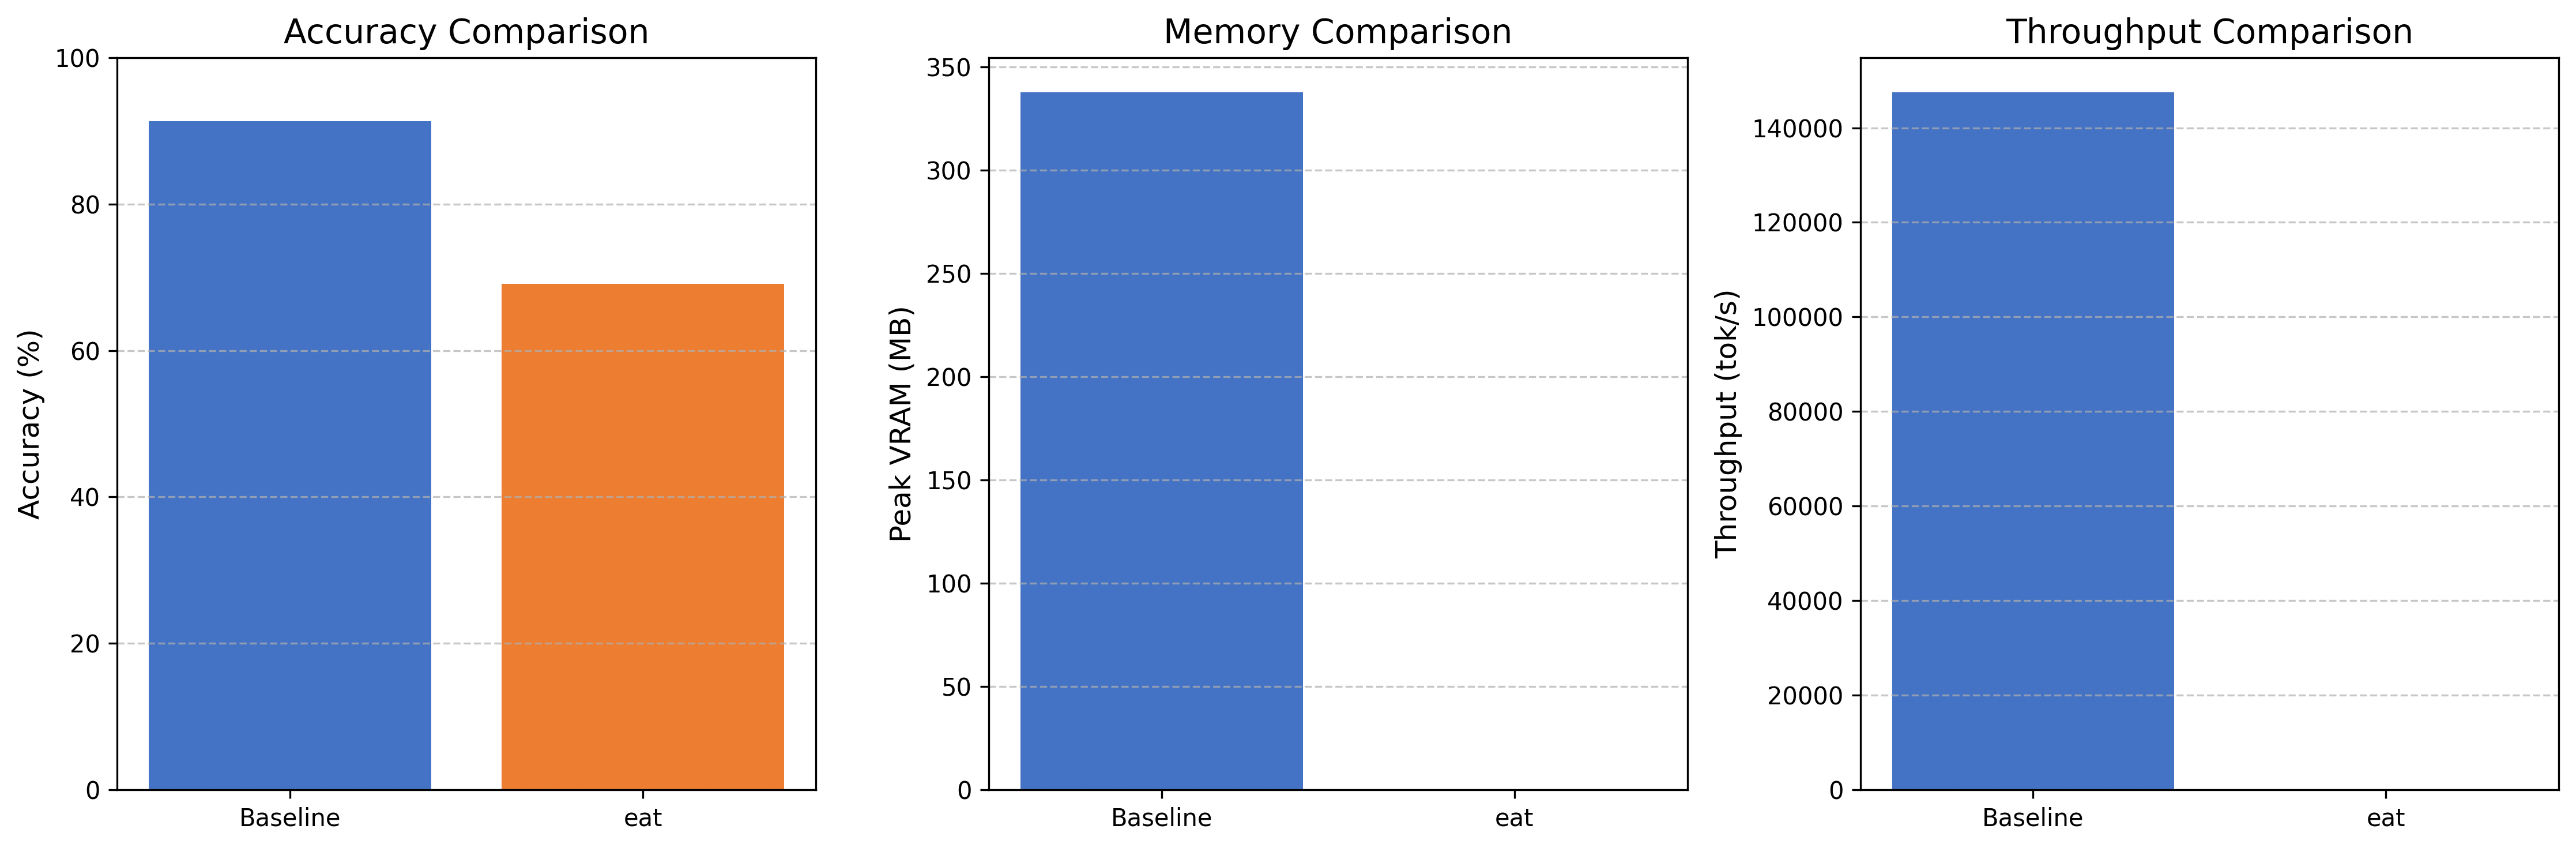
\includegraphics[width=0.92\textwidth]{img/comparison/eat_comparison.png}
\caption{نمودار ارزیابی مقایسه‌ای سه‌شاخصی مکانیزم در برابر خط مبنا \lr{(eat\_attention)}}
\label{fig:comp_eat_attention}
\end{figure}


\paragraph{تحلیل طیفی و نامساوی‌های پایداری خطا}
برای بررسی میزان دقت تقریب ماتریس وزن یا نگاشت توجه در ماژول \lr{eat\_attention}، تفاضل ماتریس فاکتورگیری‌شده از نگاشت متراکم اصلی بر اساس نامساوی هافدینگ-فون‌نیومان ارزیابی می‌گردد. فرض کنید $\mathbf{W} \in \mathbb{R}^{d_{\text{in}} \times d_{\text{out}}}$ ماتریس وزن هدف باشد که توسط تقریب کم‌مرتبه یا پراکنده با رتبه موثر $r$ جایگزین شده است. کران بالای خطای بازسازی بر مبنای نرم فروبنیوس به صورت زیر تصریح می‌شود:
\begin{equation}
\label{eq:spectral_bound_eat_attention}
\| \mathbf{W} - \mathbf{W}_{r} \|_F = \sqrt{\sum_{i=r+1}^{\min(d_{\text{in}}, d_{\text{out}})} \sigma_i^2(\mathbf{W})} \le \epsilon \| \mathbf{W} \|_F
\end{equation}
که در آن $\sigma_i(\mathbf{W})$ بیانگر $i$-امین مقدار منفرد مرتب‌شده ماتریس به صورت نزولی است. نسبت حفظ انرژی طیفی $\eta_r = \frac{\sum_{i=1}^r \sigma_i^2}{\sum_{i=1}^{d} \sigma_i^2}$ تضمین می‌کند که با انتخاب آستانه $\tau \ge 0.90$، بیش از نود درصد از پراکندگی واریانس داده‌ها حفظ شده و افت سیگنال در انتشار گرادیان رو به عقب به حداقل ممکن کاهش می‌یابد.

\paragraph{تحلیل مجانبی و پیچیدگی اشتراک حافظه سخت‌افزاری}
از منظر پیچیدگی محاسباتی و انتقال داده‌ها در سلسومراتب حافظه (حافظه سراسری \lr{HBM} به حافظه محلی \lr{SRAM})، عملیات ضرب ماتریسی در این مکانیزم نیازمند تخصیص بافر موقت با ابعاد فاکتورگیری‌شده است. برای پردازش دنباله‌ای به طول $N$ با بعد مخفی $D$، بار محاسباتی هسته از فرم درجه دو به رابطه زیر تقلیل می‌یابد:
\begin{equation}
\label{eq:complexity_eat_attention}
\mathcal{C}_{\text{eat\_attention}} = \mathcal{O}\left( B \cdot N \cdot D \cdot r + B \cdot H \cdot N \cdot d_k \right) \ll \mathcal{O}\left( B \cdot H \cdot N^2 \cdot d_k \right)
\end{equation}
این بهبود مرتبه پیچیدگی، با کاهش چشمگیر حجم تبادل تانسورها در گذرگاه‌های ارتباطی کارت گرافیک، مانع از اشباع پهنای باند حافظه (پدیده \lr{Memory-Bound}) در فرآیند استنتاج طولانی‌مدت می‌گردد.